\documentclass{article}
\usepackage{graphicx}
\usepackage[margin=1.5cm]{geometry}
\usepackage{amsmath}

\begin{document}
\twocolumn

\title{Wednesday warm-up: Forces I}
\author{Prof. Jordan C. Hanson}

\maketitle

\section{Memory Bank}

\begin{enumerate}
\item $\vec{F} = m \vec{a}$ ... Newton's 2nd Law
\item $\vec{F}_{12} = -\vec{F}_{21}$ ... Newton's 3rd Law
\item $\vec{s} = -k \Delta\vec{x}$ ... Spring force (Hooke's Law)
\end{enumerate}

\section{Chapter 4 - Forces}

\begin{enumerate}
\item If a spring with $k = 50.0$ N/m is stretched by 10 cm, what is the force $\vec{s}$?
\begin{itemize}
\item A: -500 N
\item B: 500 N
\item C: -5 N
\item D: 5 N
\end{itemize}
\item What is the force $\vec{s}$ if the spring is stretched by 5 cm?
\begin{itemize}
\item A: -250 N
\item B: 250 N
\item C: -2.5 N
\item D: 2.5 N
\end{itemize}
\item 
\begin{figure}[ht]
\centering
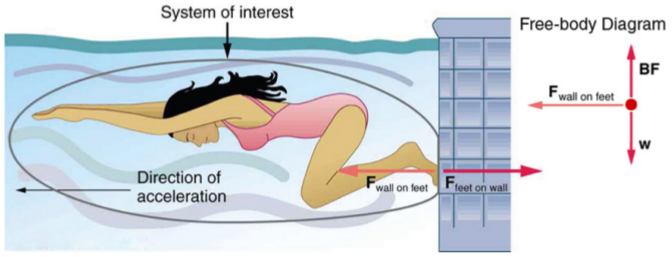
\includegraphics[width=0.45\textwidth,trim=0cm 0cm 4.75cm 2cm,clip=true]{figures/wall.png}
\caption{\label{fig:wall} A woman pushes off of a wall underwater in a pool.}
\end{figure}
According to Fig. \ref{fig:wall}, a woman experiences a force by the wall on herself.  Her weight force $w$ is balanced by the buoyant force $BF$.  (a) Draw a free body diagram for the system of interest.  (b) If the wall exerts a force of 100 N, and her mass is 50 kg, what is her acceleration? (c) Why must the wall exert a force on the woman, and not the other way around?  \\ \vspace{2.5cm}
\item 
\begin{figure}[ht]
\centering
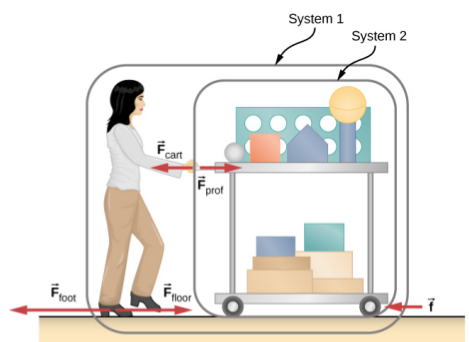
\includegraphics[width=0.45\textwidth]{figures/cart.png}
\caption{\label{fig:cart} A woman pushes off of a wall underwater in a pool.}
\end{figure}
According to Fig. \ref{fig:cart}, a professor pushes an equipment cart.  The mass of the professor is 65.0 kg, the mass of the cart is 12.0 kg, and the mass of the equipment is 7.0 kg.  The professor exerts a force of $\vec{F}_{foot} = 150.0 \hat{i}$ N on the floor.  The force of friction is $\vec{f} = -24.0\hat{i}$ N.  (a) What is the acceleration of System 1? (b) Why must we not consider $\vec{F}_{prof}$ and $\vec{F}_{cart}$ in the previous calculation? \\ \vspace{2.5cm}
\item \textit{Ay yay yay.}  A driver ran a red light, and smacked another car.  (a) Would you rather be in the \textit{lighter} vehicle, or the \textit{heavier} vehicle?  Why? (b) Suppose the mass of one car is $m_1 = 500$ kg, and the other is $m_2 = 1000$ kg.  What is the ratio of the accelerations when the cars crash?  Assume a 1D collision. (c) If the force between the cars is 2000 N, calculate the acceleration of each driver during the crash.
\end{enumerate}

\end{document}
